\documentclass[11pt,a4paper,twoside,openright,titlepage,
                           headinclude,footinclude,BCOR5mm,
                           numbers=noenddot,cleardoublepage=empty,
                           tablecaptionabove]{scrbook}
\usepackage[T1]{fontenc}
\usepackage[utf8]{inputenc}
\usepackage[italian]{babel}
\usepackage[eulerchapternumbers,beramono, pdfspacing]{classicthesis}
\usepackage{arsclassica}
\usepackage{graphicx}
\usepackage{caption}
\usepackage{subfig}
\usepackage{amsmath}
\usepackage{amsthm}
\usepackage{listings}
\definecolor{mio_colore}{RGB}{242,243,244}
\definecolor{dkgreen}{rgb}{0,0.6,0}
\definecolor{gray}{rgb}{0.5,0.5,0.5}
\lstset{language=Matlab,basicstyle=\small\ttfamily,showstringspaces=false,numberstyle=\tiny\color{gray}, keywordstyle=\color{blue},commentstyle=\color{dkgreen},stringstyle=\color{red}, backgroundcolor=\color{mio_colore}}

\begin{document}
\section*{Esercizio L}
La funzione \emph{L6} è:
\begin{lstlisting}[frame=trBL]
function [b] = L6(a)
% applichiamo il filtro 
% dell'esercizio L6 
% all'immagine salvata in a
s=size(a);
m=s(1);
n=s(2);
k=floor(m/2);
u=[1:k];
f=(1-cos((3*pi/2)+(2*pi/m)*u)).^3;
if (mod(m,2)==0)
    f1=[1,f,f(k-1:-1:1)];
else
    f1=[1,f,f(k:-1:1)];
end

k=floor(n/2);
u=[1:k];
f=(1-cos((3*pi/2)+(2*pi/n)*u)).^3;
if (mod(n,2)==0)
    f2=[1,f,f(k-1:-1:1)];
else
    f2=[1,f,f(k:-1:1)];
end
b = double(a);
for i=1:3
    v = fft2(double(a(:,:,i)));
    v = diag(f1)*v*diag(f2);
    v=ifft2(v);
    b(:,:,i)=real(v);
end
mx=max(max(max(b)));
fattore = 250.0/mx;
b = b*fattore;
b = uint8(b);
% imshow(b);
end
\end{lstlisting}
Applicandola all'immagine \emph{fox.png}
\begin{figure}[h!]
\centering

\includegraphics[width=.25\textwidth]{figs/fox.jpg} 
\caption{Immagine di esempio.}
\end{figure}
\newpage
si ottiene:
\begin{figure}[h!]
\centering

\includegraphics[width=.45\textwidth]{figs/fox_filtrata.jpg} 
\caption{Immagine filtrata.}
\end{figure}
\newpage

\section*{Esercizio M}
La funzione \emph{M6} è:
\begin{lstlisting}[frame=trBL]
function [B] = M6(A)

[m, n, ~] = size(A);
B = 9*A;
B(1:m-1,:,:) = B(1:m-1,:,:)-A(2:m,:,:); 
B(2:m,:,:) = B(2:m,:,:)-A(1:m-1,:,:);
B(:,1:n-1,:) = B(:,1:n-1,:)-A(:,2:n,:);
B(:,2:n,:) = B(:,2:n,:)-A(:,1:n-1,:);
B(1:m-1,1:n-1,:) = B(1:m-1,1:n-1,:)+A(2:m,2:n,:);
B(1:m-1,2:n,:) = B(1:m-1,2:n,:)+A(2:m,1:n-1,:);
B(2:m,2:n,:) = B(2:m,2:n,:)+A(1:m-1,1:n-1,:);
B(2:m,1:n-1,:) = B(2:m,1:n-1,:)+A(1:m-1,2:n,:);

end
\end{lstlisting}

Applicandola all'immagine \emph{mimosa.png}
\begin{figure}[h!]
\centering
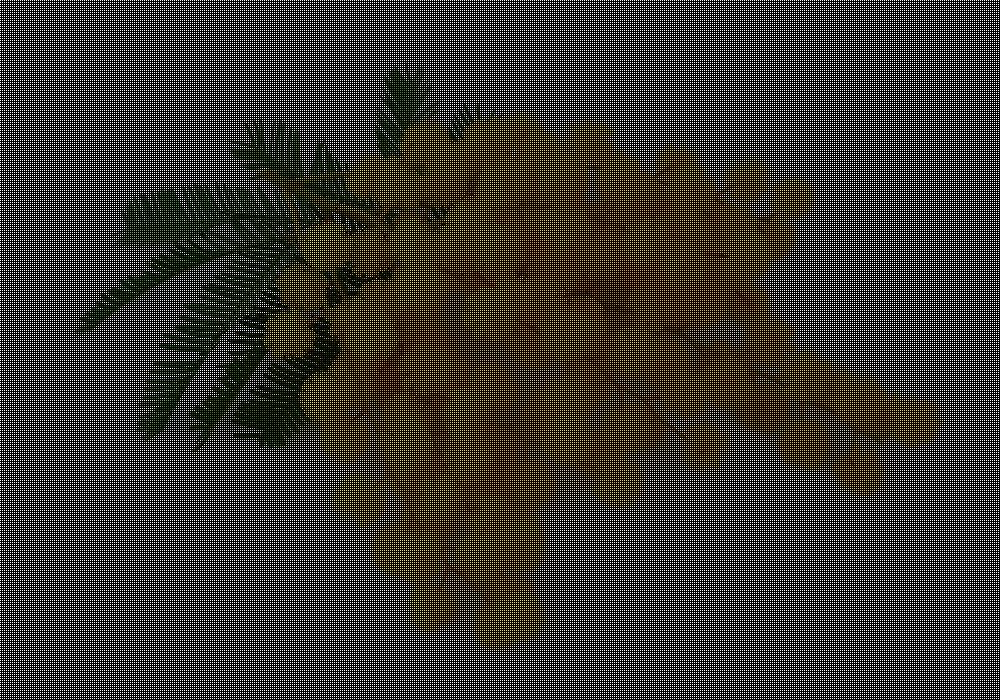
\includegraphics[width=.45\textwidth]{figs/mimosa.jpg} 
\caption{Immagine di esempio.}
\end{figure}
\par
si ottiene:
\begin{figure}[h!]
\centering
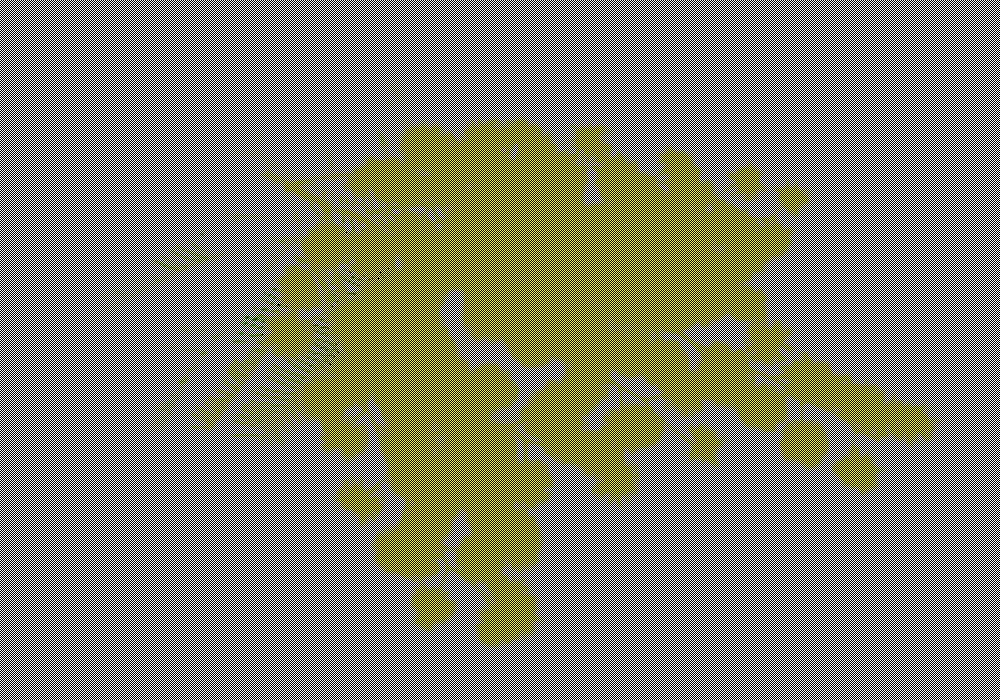
\includegraphics[width=.45\textwidth]{figs/mimosa_filtrata.jpg} 
\caption{Immagine filtrata.}
\end{figure}


\end{document}
